\def\rot{\rotatebox}
\newcolumntype{a}{>{\columncolor{gr1}}r}
\newcolumntype{b}{>{\columncolor{gr2}}r}
\newcolumntype{c}{>{\columncolor{gr3}}r}
\newcolumntype{d}{>{\columncolor{gr4}}r}
\begin{figure}[!htbp]
\centering 
% \subfloat[subfig:plans][Defects Reduced. \textit{Higher defect reduction} for larger overlap is considered \textit{better}.]{
% \arrayrulecolor[gray]{0.5}
% \resizebox{\linewidth}{!}{
% \begin{tabular}{@{}l|rrra|rrrb|rrrc|rrrd}
%             \rowcolor{white}& \multicolumn{4}{c|}{$0\leq Overlap<25$}       & \multicolumn{4}{c|}{$25\leq Overlap<50$}       & \multicolumn{4}{c|}{$50\leq Overlap<75$}       & \multicolumn{4}{c}{$75\leq Overlap\leq100$}      \bigstrut \\ \hline
%             & \rot{90}{ALVES} & \rot{90}{OLIVE} & \rot{90}{SHATW~~} & \cellcolor{white}\rot{90}{XTREE} & \rot{90}{ALVES} & \rot{90}{OLIVE} & \rot{90}{SHATW~~} & \cellcolor{white}\rot{90}{XTREE} & \rot{90}{ALVES} & \rot{90}{OLIVE} & \rot{90}{SHATW~~} & \cellcolor{white}\rot{90}{XTREE} & \rot{90}{ALVES} & \rot{90}{OLIVE} & \rot{90}{SHATW~~} & \cellcolor{white}\rot{90}{XTREE} \bigstrut \\ \hline
% ant-1      & 3  & 2  & 13  & 13 & 6  & 7  & 3   & 33  & 1  & 2  & 0  & 27  & 2  & 3   & 0 & 62  \bigstrut \\
% ant-2      & 0  & 1  & 0   & 6  & 6  & 5  & 0   & 42  & 0  & 2  & 0  & 27  & 0  & 0   & 0 & 124 \bigstrut \\
% ant-3      & 10 & 6  & 22  & 18 & 16 & 15 & 1   & 71  & 2  & 5  & 0  & 47  & 0  & 1   & 0 & 108 \bigstrut \\ \hline
% camel-1    & 17 & 8  & 76  & 29 & 22 & 25 & 0   & 90  & 28 & 10 & 0  & 52  & 17 & 38  & 0 & 226 \bigstrut \\
% camel-2    & 9  & 3  & 36  & 25 & 21 & 17 & 0   & 109 & 18 & 11 & 0  & 69  & 0  & 18  & 0 & 439 \bigstrut \\ \hline
% ivy-1      & 1  & 1  & 1   & 4  & 0  & 0  & 0   & 10  & 0  & 0  & 0  & 5   & 0  & 0   & 0 & 12  \bigstrut \\ \hline
% jedit-1    & 9  & 5  & 13  & 9  & 7  & 6  & 8   & 35  & 5  & 7  & 0  & 39  & 0  & 3   & 0 & 136 \bigstrut \\
% jedit-2    & 14 & 7  & 28  & 24 & 10 & 14 & 1   & 77  & 4  & 2  & 0  & 36  & 0  & 2   & 0 & 107 \bigstrut \\ 
% jedit-3    & 14 & 10 & 18  & 30 & 4  & 6  & 1   & 67  & 1  & 1  & 0  & 28  & 0  & 1   & 0 & 70  \bigstrut \\ \hline
% log4j-1    & 2  & 0  & 5   & 1  & 1  & 3  & 0   & \cellcolor{white}7   & 1  & 0  & 0  & \cellcolor{white}3   & 0  & 1   & 0 & \cellcolor{white}8   \bigstrut \\ \hline
% lucene-1   & 8  & 2  & 21  & 6  & 17 & 17 & 19  & 36  & 13 & 5  & 0  & 17  & 1  & 15  & 0 & \cellcolor{white}57  \bigstrut \\ \hline
% poi-1      & 0  & 0  & 1   & \cellcolor{white}0  & 0  & 0  & 5   & \cellcolor{white}0   & 6  & 0  & 0  & \cellcolor{white}2   & 0  & 6   & 0 & \cellcolor{white}81  \bigstrut \\
% poi-2      & 49 & 2  & 78  & 4  & 32 & 72 & 18  & 135 & 15 & 12 & 0  & 27  & 0  & 16  & 0 & 87  \bigstrut \\ \hline
% velocity-1 & 9  & 2  & 51  & 2  & 26 & 12 & 0   & 25  & 11 & 15 & 0  & 39  & 4  & 24  & 0 & 90  \bigstrut \\ \hline
% xalan-1    & 4  & 2  & 22  & 6  & 27 & 19 & 105 & \cellcolor{white}43  & 70 & 21 & 13 & 60  & 38 & 103 & 0 & 409 \bigstrut \\
% xalan-2    & 7  & 0  & 110 & \cellcolor{white}0  & 63 & 18 & 0   & 38  & 51 & 53 & 0  & 102 & 4  & 56  & 0 & \cellcolor{white}83  \bigstrut \\ \hline
% xerces-1   & 2  & 1  & 23  & 2  & 6  & 3  & 0   & \cellcolor{white}11  & 9  & 3  & 0  & 17  & 7  & 18  & 0 & 305 \bigstrut \\
% xerces-2   & 0  & 0  & 7   & \cellcolor{white}0  & 1  & 1  & 0   & \cellcolor{white}3   & 6  & 2  & 0  & \cellcolor{white}6   & 1  & 6   & 0 & \cellcolor{white}117  
% \end{tabular}}
% \label{subfig:rq2_dec}}\\
% \subfloat[subfig:plans][Defects Increased. In comparison to defects reduced in \fig{rq2}(a) above, we would like to have as little defects increased as possible.]{
% \arrayrulecolor[gray]{0.5}
% \resizebox{\linewidth}{!}{
% \begin{tabular}{@{}l|rrra|rrrb|rrrc|rrrd}
%             \rowcolor{white}& \multicolumn{4}{c|}{$0\leq Overlap<25$}       & \multicolumn{4}{c|}{$25\leq Overlap<50$}       & \multicolumn{4}{c|}{$50\leq Overlap<75$}       & \multicolumn{4}{c}{$75\leq Overlap\leq100$}      \bigstrut \\ \hline
%             & \rot{90}{ALVES} & \rot{90}{OLIVE} & \rot{90}{SHATW~~} & \cellcolor{white}\rot{90}{XTREE} & \rot{90}{ALVES} & \rot{90}{OLIVE} & \rot{90}{SHATW~~} & \cellcolor{white}\rot{90}{XTREE} & \rot{90}{ALVES} & \rot{90}{OLIVE} & \rot{90}{SHATW~~} & \cellcolor{white}\rot{90}{XTREE} & \rot{90}{ALVES} & \rot{90}{OLIVE} & \rot{90}{SHATW~~} & \cellcolor{white}\rot{90}{XTREE} \bigstrut \\ \hline
% ant-1      & 15  & 15  & 15  & 1  & 0  & 0  & 0  & 10 & 0  & 0  & 0 & 2  & 0 & 0  & 0 & 4   \bigstrut\\
% ant-2      & 59  & 58  & 63  & 9  & 4  & 4  & 0  & 33 & 0  & 0  & 0 & 11 & 0 & 0  & 0 & 20  \bigstrut\\
% ant-3      & 66  & 64  & 69  & 22 & 4  & 7  & 0  & 38 & 0  & 0  & 0 & 15 & 0 & 0  & 0 & 10  \bigstrut\\\hline
% camel-1    & 29  & 28  & 36  & 10 & 5  & 5  & 0  & 11 & 2  & 2  & 0 & 6  & 0 & 0  & 0 & 14  \bigstrut\\
% camel-2    & 102 & 97  & 112 & 5  & 10 & 9  & 0  & 26 & 4  & 3  & 0 & 17 & 0 & 4  & 0 & 74  \bigstrut\\\hline
% ivy-1      & 6   & 6   & 6   & 1  & 0  & 0  & 0  & 3  & 0  & 0  & 0 & 2  & 0 & 0  & 0 & 0   \bigstrut\\\hline
% jedit-1    & 37  & 33  & 37  & 3  & 3  & 5  & 2  & 20 & 1  & 1  & 0 & 11 & 0 & 1  & 0 & 12  \bigstrut\\
% jedit-2    & 14  & 12  & 15  & 2  & 1  & 2  & 0  & 8  & 0  & 0  & 0 & 2  & 0 & 0  & 0 & 4   \bigstrut\\
% jedit-3    & 3   & 2   & 3   & 1  & 0  & 0  & 0  & 1  & 0  & 0  & 0 & 1  & 0 & 0  & 0 & 0   \bigstrut\\\hline
% log4j-1    & 68  & 66  & 73  & 1  & 3  & 4  & 1  & \cellcolor{white}14 & 3  & 2  & 0 & \cellcolor{white}13 & 0 & 2  & 0 & \cellcolor{white}47 \bigstrut\\\hline
% lucene-1   & 75  & 72  & 85  & 3  & 17 & 10 & 10 & 30 & 7  & 5  & 0 & 11 & 0 & 9  & 0 & \cellcolor{white}54 \bigstrut\\\hline
% poi-1      & 189 & 186 & 190 & \cellcolor{white}1  & 3  & 2  & 6  & \cellcolor{white}7  & 5  & 1  & 0 & \cellcolor{white}5  & 0 & 6  & 0 & \cellcolor{white}182 \bigstrut\\
% poi-2      & 84  & 78  & 87  & 4  & 8  & 9  & 2  & 23 & 0  & 2  & 0 & 11 & 0 & 0  & 0 & 58 \bigstrut\\\hline
% velocity-1 & 15  & 13  & 21  & 1  & 1  & 2  & 4  & 3  & 4  & 1  & 0 & 3  & 1 & 4  & 0 & 14 \bigstrut\\\hline
% xalan-1    & 144 & 142 & 152 & 2  & 15 & 9  & 21 & \cellcolor{white}46 & 13 & 8  & 6 & 33 & 4 & 13 & 0 & 101 \bigstrut\\
% xalan-2    & 460 & 452 & 506 & \cellcolor{white}27 & 26 & 5  & 0  & 25 & 35 & 33 & 0 & 87 & 0 & 18 & 0 & \cellcolor{white}388\bigstrut\\\hline
% xerces-1   & 49  & 47  & 52  & 0  & 1  & 2  & 0  & \cellcolor{white}10 & 1  & 1  & 0 & 11 & 0 & 0  & 0 & 34  \bigstrut\\
% xerces-2   & 163 & 161 & 169 & \cellcolor{white}4  & 6  & 5  & 0  & \cellcolor{white}14 & 1  & 2  & 0 & \cellcolor{white}9  & 0 & 1  & 0 & \cellcolor{white}146
% \end{tabular}}
% \label{fig:rq2_inc}
% }
\subfloat[Defects Reduced]{
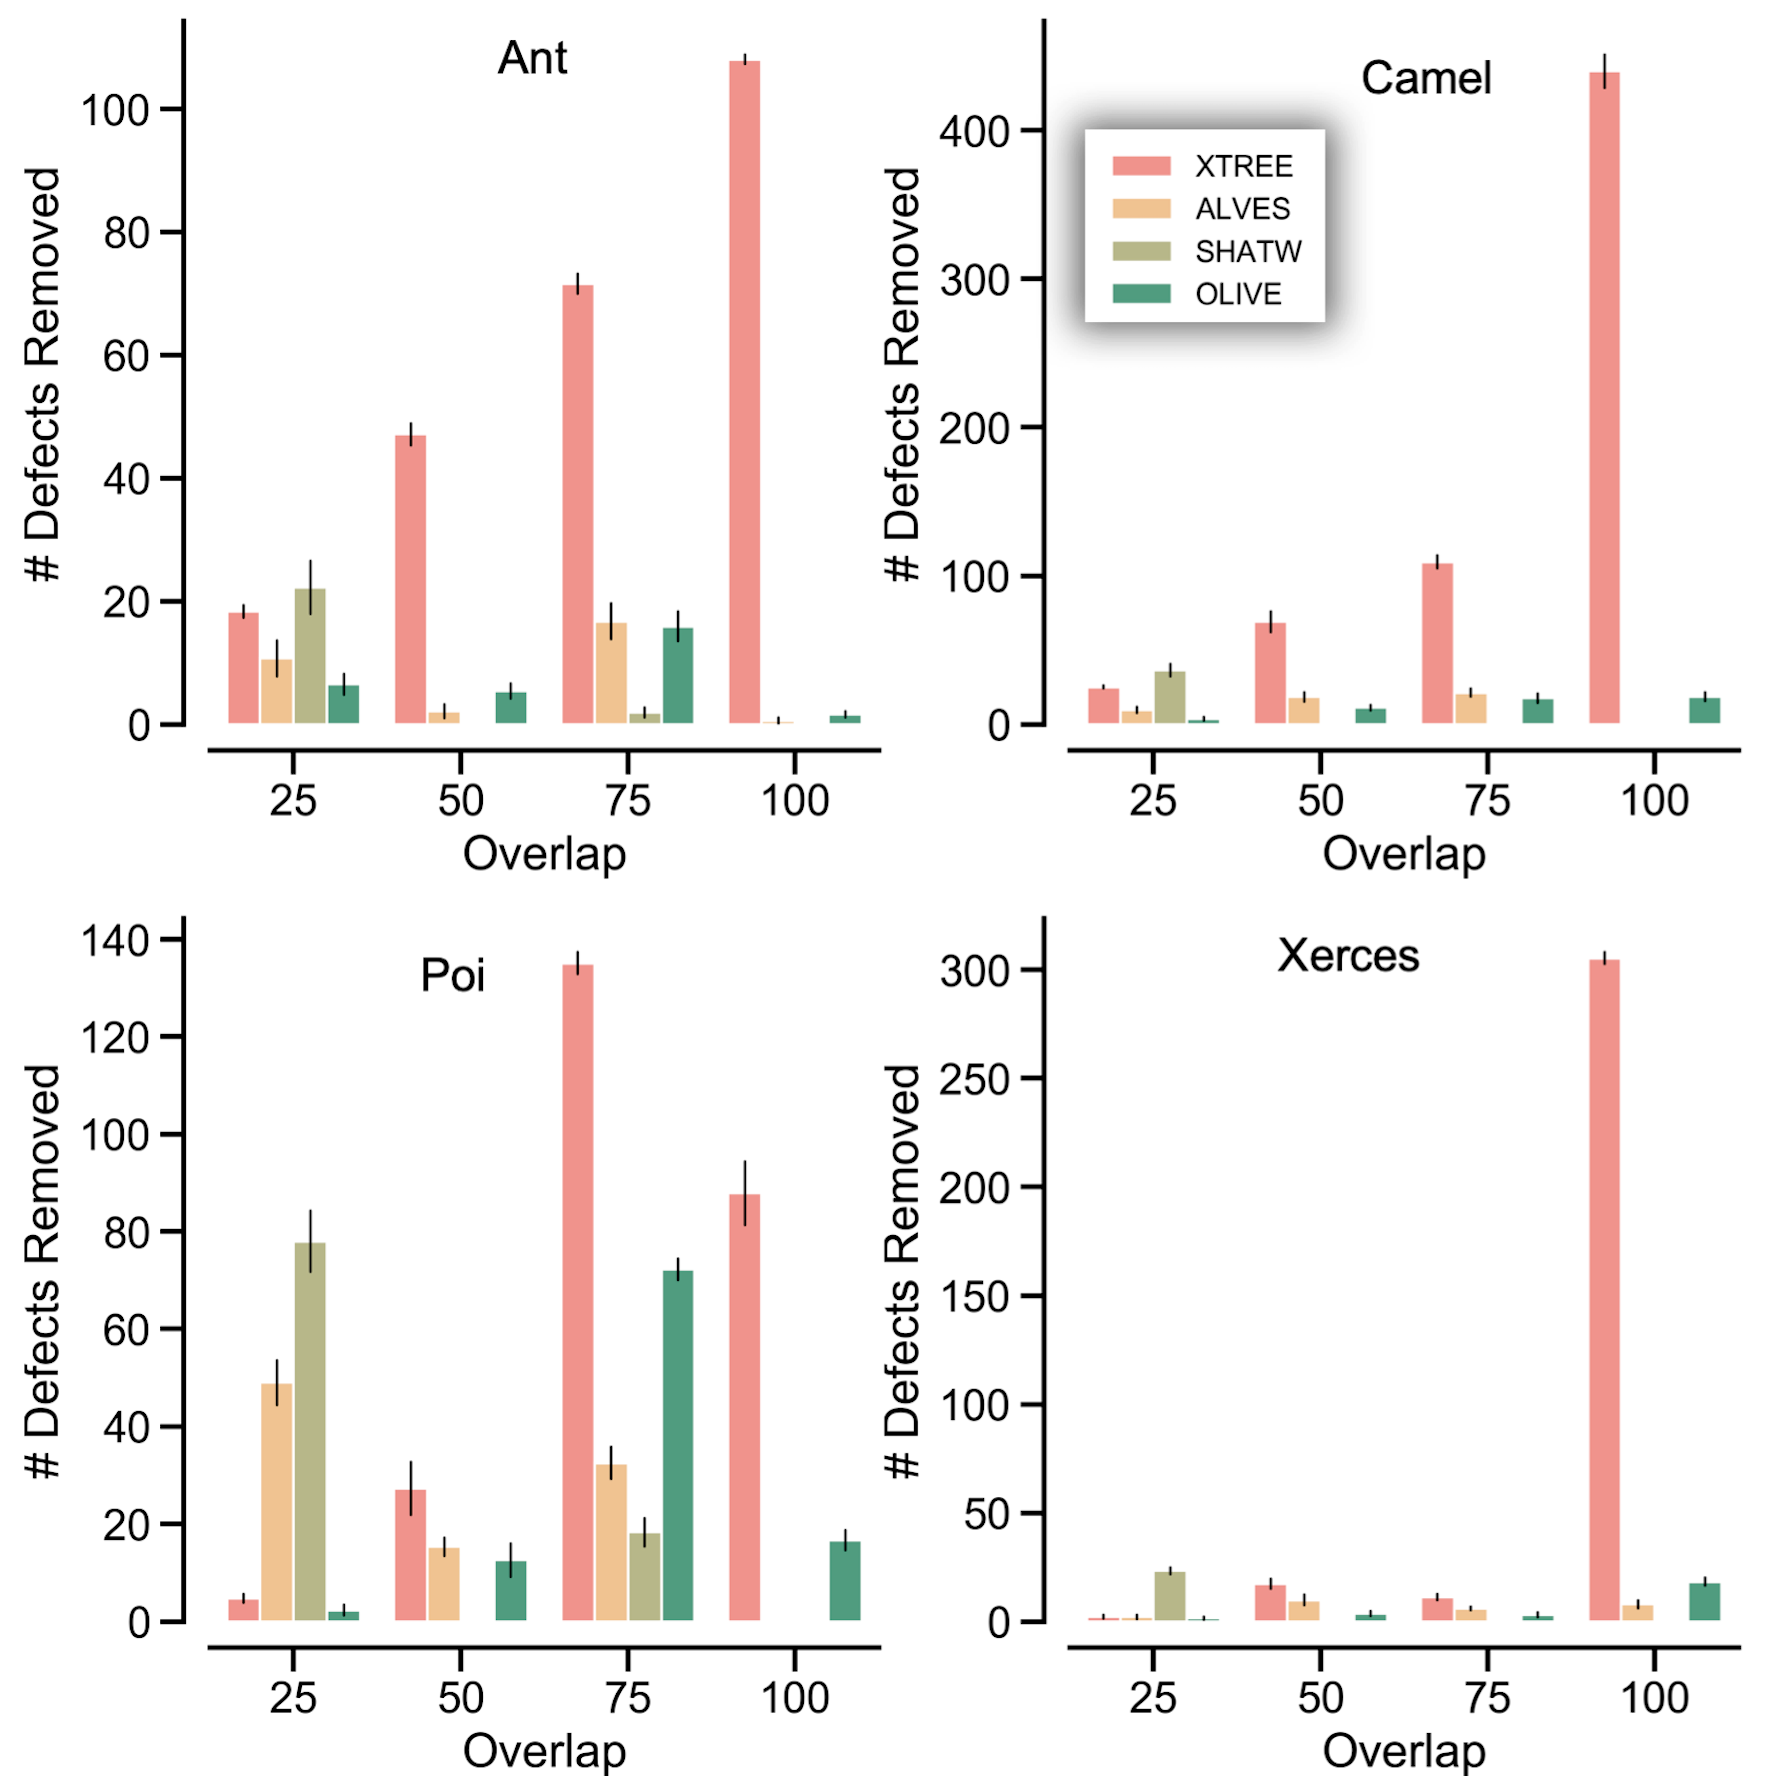
\includegraphics[width=0.75\linewidth]{rq2_1.png}
\label{fig:rq2_a}}\\~\hrule~
\subfloat[Defects Increased]{
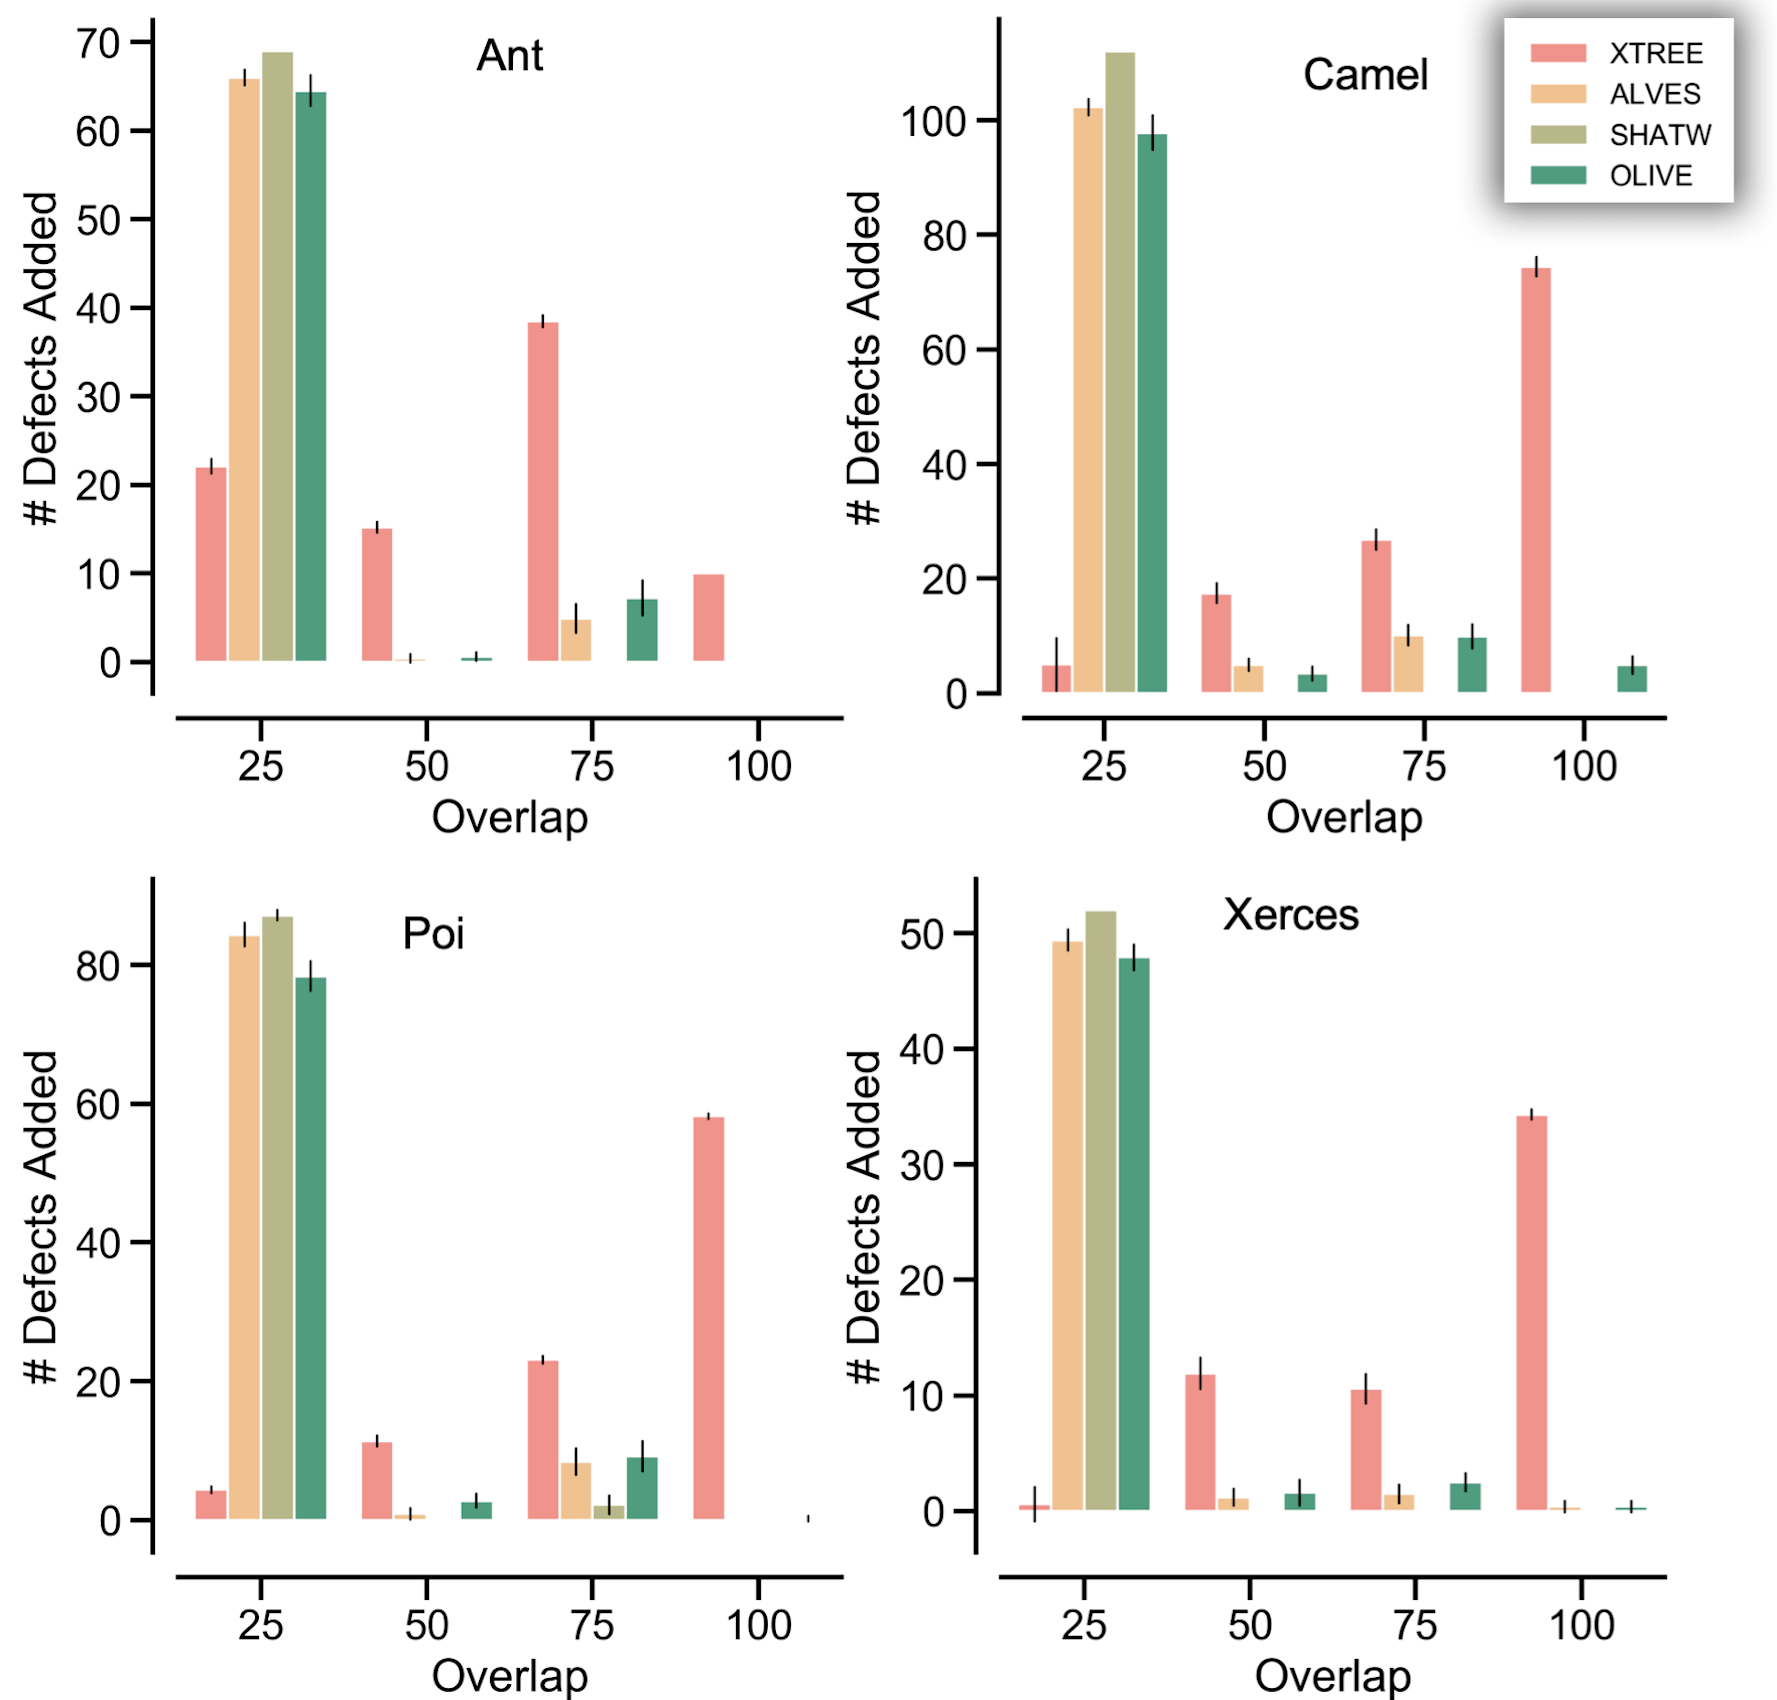
\includegraphics[width=0.75\linewidth]{rq2_2.png}
\label{fig:rq2_b}}
\caption{A count of total number \textit{defects reduced} and \textit{defects increased} as a result each planners' recommendations. The overlaps are again categorized into four ranges for every dataset (denoted by $min\leq~Overlap<max$). For each of the overlap ranges, we count the total number of \textit{defects reduced} and \textit{defects increased} in the validation set for the classes that were defective in the test set as a result of overlap between the planner's recommendation and the developers changes that fell in the given range}
\label{fig:rq2}
\end{figure}